Sea $\ket{\psi}=\alpha\ket{0}+\beta\ket{1}$ con $|\alpha|^2+|\beta|^2=1$. Se busca un estado
$\ket{\psi'}=\alpha'\ket{0}+\beta'\ket{1}$ con las mismas probabilidades de medición. Por la regla de Born, esas probabilidades son $|\alpha|^2$ y $|\beta|^2$, donde $|z|=\sqrt{a^2+b^2}$ es el \emph{módulo} de $z=a+ib$, es decir, su tamaño o distancia al origen del plano complejo. Tener las mismas probabilidades significa, entonces,
$|\alpha'|=|\alpha|$ y $|\beta'|=|\beta|$. Se busca además un $\eta\in\mathbb{R}$ tal que
$\ket{\psi}+e^{i\eta}\ket{\psi'}=c\ket{1}$ con $c\neq0$. Agrupando los coeficientes de $\ket0$ y
$\ket1$,
\begin{equation}\label{eq:13-suma}
  \ket{\psi}+e^{i\eta}\ket{\psi'}
  =\bigl(\alpha+e^{i\eta}\alpha'\bigr)\ket{0}+\bigl(\beta+e^{i\eta}\beta'\bigr)\ket{1}.
\end{equation}
Como $c\ket1=0\cdot\ket0+c\cdot\ket1$ y dos vectores son iguales si y solo si tienen las mismas
coordenadas en la base $\{\ket0,\ket1\}$,
\begin{equation}\label{eq:13-sistema}
  \destacado{\alpha+e^{i\eta}\alpha'=0,\qquad \beta+e^{i\eta}\beta'=c.}
\end{equation}
En cada ecuación se suman dos amplitudes del mismo resultado de medición. En la primera, la suma
debe ser cero: el resultado $0$ desaparece aunque cada estado por separado lo da con probabilidad
$|\alpha|^2$. Esto no puede pasar con probabilidades, porque $|\alpha|^2+|\alpha|^2>0$ si
$\alpha\neq0$, pero sí con amplitudes, porque dos números complejos distintos de cero pueden
sumar cero. Esa cancelación es la interferencia.

De la primera ecuación, $\alpha+e^{i\eta}\alpha'=0$, se obtiene $\alpha'=-e^{-i\eta}\alpha$, y
como el módulo de un producto es el producto de los módulos, $|zw|=|z|\,|w|$, y $|e^{-i\eta}|=\sqrt{\cos^2\eta+\sin^2\eta}=1$, se tiene $|\alpha'|=|\alpha|$ para cualquier $\eta$. De la segunda,
$\beta+e^{i\eta}\beta'=c$, se obtiene $c-\beta=e^{i\eta}\beta'$, y tomando módulos,
$|c-\beta|=|e^{i\eta}|\,|\beta'|=|\beta'|$. El número $|c-\beta|$ es la distancia entre los puntos $c$ y $\beta$ del plano complejo. Como se pide $|\beta'|=|\beta|$, el número $c$ debe cumplir
\begin{equation}\label{eq:13-circulo}
  \destacado{|c-\beta|=|\beta|,\qquad c\neq 0,}
\end{equation}
es decir, $c$ está en la circunferencia de centro $\beta$ y radio $|\beta|$, sin el origen
(figura~\ref{fig:13-circulo}). Esa circunferencia siempre pasa por el origen, porque
$|0-\beta|=|\beta|$.

\subsection*{Existencia}

Si $\beta=0$, la circunferencia $|c-\beta|=|\beta|$ \eqref{eq:13-circulo} se reduce al punto
$c=0$, que está excluido, así que no hay solución. En ese caso $\ket\psi$ es $\ket0$ salvo fase
global, y al cancelar su amplitud de $\ket0$ no queda nada. Si $\beta\neq0$, cualquier $c\neq0$
de la circunferencia da una solución:
\begin{equation}\label{eq:13-construccion}
  \alpha'=-e^{-i\eta}\alpha,\qquad \beta'=e^{-i\eta}(c-\beta)
\end{equation}
cumplen $|\alpha'|=|\alpha|$, $|\beta'|=|c-\beta|=|\beta|$ y las dos ecuaciones
$\alpha+e^{i\eta}\alpha'=0$, $\beta+e^{i\eta}\beta'=c$ de \eqref{eq:13-sistema}. Por tanto,
\[
  \destacado{\text{existe }\ket{\psi'}\iff \beta\neq0\iff \ket\psi\text{ no es }\ket0
  \text{ salvo fase global}.}
\]

\subsection*{Todas las soluciones y la unicidad}

Para nombrar cada punto de la circunferencia se usa que $c-\beta$ y $\beta$ tienen el mismo
módulo $B=|\beta|$. En forma polar (punto 1.1), $\beta=Be^{iy}$ y $c-\beta=Be^{iy'}$ para algún
ángulo $y'$, así que solo difieren en el ángulo. Si $\tau\in(-\pi,\pi]$ es esa diferencia,
$\tau\equiv y'-y\pmod{2\pi}$ (es decir, $\tau$ es el ángulo de $(-\pi,\pi]$ que difiere de $y'-y$ en un múltiplo entero de $2\pi$; véase el punto 1.2), entonces $c-\beta=e^{i(y'-y)}Be^{iy}=e^{i\tau}\beta$: el número
$c-\beta$ es $\beta$ girado un ángulo $\tau$. Por tanto,
\begin{equation}\label{eq:13-c-tau}
  \destacado{c=\beta\bigl(1+e^{i\tau}\bigr),\qquad \tau\in(-\pi,\pi],}
\end{equation}
y cada $\tau$ da un punto distinto de la circunferencia. Con $\tau=\pi$ se obtiene $c=0$, que
está excluido. Al reemplazar $c-\beta=e^{i\tau}\beta$ en $\alpha'=-e^{-i\eta}\alpha$, $\beta'=e^{-i\eta}(c-\beta)$ \eqref{eq:13-construccion}, se obtiene $\beta'=e^{-i\eta}e^{i\tau}\beta$, y sacando el factor común $e^{-i\eta}$, todas las
soluciones son
\begin{equation}\label{eq:13-soluciones}
  \destacado{\ket{\psi'}=e^{-i\eta}\bigl(-\alpha\ket0+e^{i\tau}\beta\ket1\bigr),
  \qquad \eta\in\mathbb R,\quad \tau\in(-\pi,\pi).}
\end{equation}
Es decir, $\ket{\psi'}$ se obtiene de $\ket\psi$ cambiando el signo de $\alpha$ y girando $\beta$
un ángulo $\tau$. El factor $e^{-i\eta}$ es una fase global (punto 1.2) y no cambia el estado,
pero cada $\tau$ da un estado distinto, así que \textbf{la solución no es única}: hay una por
cada $\tau\in(-\pi,\pi)$. El valor excluido $\tau=\pi$ daría $\ket{\psi'}=-e^{-i\eta}\ket\psi$,
el mismo $\ket\psi$; en ese caso también se cancelaría la amplitud de $\ket1$. Si $\alpha=0$,
no hay nada que cancelar y la única solución es $\ket\psi=\ket1$ salvo fase global; en lo que
sigue se supone $\alpha\neq0$ y $\beta\neq0$.

\subsection*{Cómo depende $c$ de $\ket\psi$}

Por $c=\beta(1+e^{i\tau})$ \eqref{eq:13-c-tau}, $c$ depende de $\ket\psi$ solo a través de
$\beta$, el coeficiente de $\ket1$; el coeficiente $\alpha$ no interviene. Para su módulo, con
$e^{i\tau}=\cos\tau+i\sin\tau$,
\[
  |1+e^{i\tau}|^2=(1+\cos\tau)^2+\sin^2\tau=2+2\cos\tau,
  \qquad\text{así que}\qquad
  \destacado{|c|=|\beta|\sqrt{2+2\cos\tau}.}
\]
El módulo es máximo, $|c|=2|\beta|$, con $\tau=0$, cuando las dos amplitudes de $\ket1$ son
iguales y se suman completas; esa solución es $\ket{\psi'}=-\alpha\ket0+\beta\ket1$. Cuando
$\tau\to\pm\pi$, las dos amplitudes de $\ket1$ se vuelven opuestas y $|c|\to0$. En todos los
casos, al normalizar la suma queda $\frac{c}{|c|}\ket1$, que es $\ket1$ salvo fase global: el
estado final es el mismo para todas las soluciones y solo cambia el tamaño $|c|$ antes de
normalizar.

\subsection*{Interpretación en la esfera de Bloch}

La altura del punto de un estado en la esfera de Bloch es $|\alpha|^2-|\beta|^2$, así que dos
estados con las mismas probabilidades están en el mismo paralelo (la misma circunferencia
horizontal). Las soluciones $\ket{\psi'}$ están entonces en el paralelo de $\ket\psi$, y con
$\varphi\equiv y-x$ \eqref{eq:phi}, su longitud es
$\varphi'\equiv(y+\tau)-(x+\pi)=\varphi+\tau-\pi$, que nunca es $\varphi$ porque $\tau\neq\pi$.
Por tanto, las soluciones son todos los puntos del paralelo de $\ket\psi$ excepto $\ket\psi$, y
la suma normalizada siempre es el polo sur, $\ket1$: ese estado tiene $A=0$ y $B=1$, así que $\cos\frac\theta2=0$, $\theta=\pi$, y su punto es $\vec r=(0,0,A^2-B^2)=(0,0,-1)$. Como una fase global no mueve el punto, $\frac{c}{|c|}\ket1$ queda en el mismo polo sur para cualquier $\tau$. La solución con mayor $|c|$ ($\tau=0$,
$\varphi'=\varphi-\pi$) es el punto del paralelo opuesto a $\ket\psi$.

\subsection*{Comprobación con el widget}

Para $\ket\psi=\frac{\sqrt3}{2}\ket0+\frac{i}{2}\ket1$ ($\theta=60^\circ$, $\varphi=90^\circ$,
figura~\ref{fig:13-widget-psi}) y $\eta=0$, las soluciones son $\ket{\psi'}=-\frac{\sqrt3}{2}\ket0+\frac{i}{2}e^{i\tau}\ket1$.
Tres de ellas:
\begin{center}
\renewcommand{\arraystretch}{1.4}
\begin{tabular}{ccccc}
  $\tau$ & $\ket{\psi'}$ & $\varphi'$ & $c=\beta(1+e^{i\tau})$ & $|c|$\\\hline
  $0$ & $-\frac{\sqrt3}{2}\ket0+\frac{i}{2}\ket1$ & $-90^\circ$ & $i$ & $1$\\
  $\frac\pi2$ & $-\frac{\sqrt3}{2}\ket0-\frac12\ket1$ & $0^\circ$ & $-\frac12+\frac{i}{2}$ & $\frac{\sqrt2}{2}$\\
  $-\frac\pi2$ & $-\frac{\sqrt3}{2}\ket0+\frac12\ket1$ & $180^\circ$ & $\frac12+\frac{i}{2}$ & $\frac{\sqrt2}{2}$
\end{tabular}
\end{center}
Por ejemplo, con $\tau=\frac\pi2$,
$\ket\psi+\ket{\psi'}=\bigl(\frac{i}{2}-\frac12\bigr)\ket1$, así que $c=-\frac12+\frac{i}{2}$ y
$|c|=\frac{\sqrt2}{2}=\frac12\sqrt{2+2\cos\frac\pi2}$. En el widget
(figura~\ref{fig:13-widget-bloch}) los cuatro estados tienen la misma altura, $r_z=0.5$, y solo
cambia la longitud; el estado final es el polo sur.

\begin{figure}[H]
\centering
\begin{tikzpicture}[scale=2.6, line cap=round]
  \draw[black!12] (-0.75,-0.25) grid[step=0.25] (0.75,1.15);
  \draw[-{Stealth[length=2mm]}, black!60] (-0.85,0) -- (0.95,0) node[right, font=\footnotesize]{Re};
  \draw[-{Stealth[length=2mm]}, black!60] (0,-0.3) -- (0,1.25) node[above, font=\footnotesize]{Im};
  \draw[resaltado!70, thick] (0,0.5) circle (0.5);
  \draw[very thick, colSu] (0,0) -- (0,0.5);
  \fill[colSu] (0,0.5) circle (0.022) node[anchor=south west, font=\footnotesize, xshift=1pt, yshift=1pt]{$\beta=\frac{i}{2}$};
  \draw[colSu, densely dashed, -{Stealth[length=1.6mm]}] (0,0.5) -- (0,0.98);
  \draw[colSu, densely dashed, -{Stealth[length=1.6mm]}] (0,0.5) -- (-0.48,0.5);
  \draw[colSu, densely dashed, -{Stealth[length=1.6mm]}] (0,0.5) -- (0.48,0.5);
  \fill[resaltado] (0,1) circle (0.026) node[above right, font=\scriptsize]{$\tau=0$: $c=i$};
  \fill[resaltado] (-0.5,0.5) circle (0.026) node[left, font=\scriptsize]{$\tau=\frac\pi2$: $c=-\frac12+\frac{i}{2}$};
  \fill[resaltado] (0.5,0.5) circle (0.026) node[right, font=\scriptsize]{$\tau=-\frac\pi2$: $c=\frac12+\frac{i}{2}$};
  \filldraw[fill=white, draw=resaltado, thick] (0,0) circle (0.028);
  \node[font=\scriptsize, resaltado, anchor=north west] at (0.03,-0.02) {$\tau=\pi$: $c=0$ (excluido)};
\end{tikzpicture}
\caption{Valores posibles de $c$ en el ejemplo: la circunferencia de centro $\beta$ y radio
$|\beta|$. Cada flecha punteada es $c-\beta=e^{i\tau}\beta$, es decir, $\beta$ girado un
ángulo $\tau$.}
\label{fig:13-circulo}
\end{figure}

\begin{figure}[H]
\centering
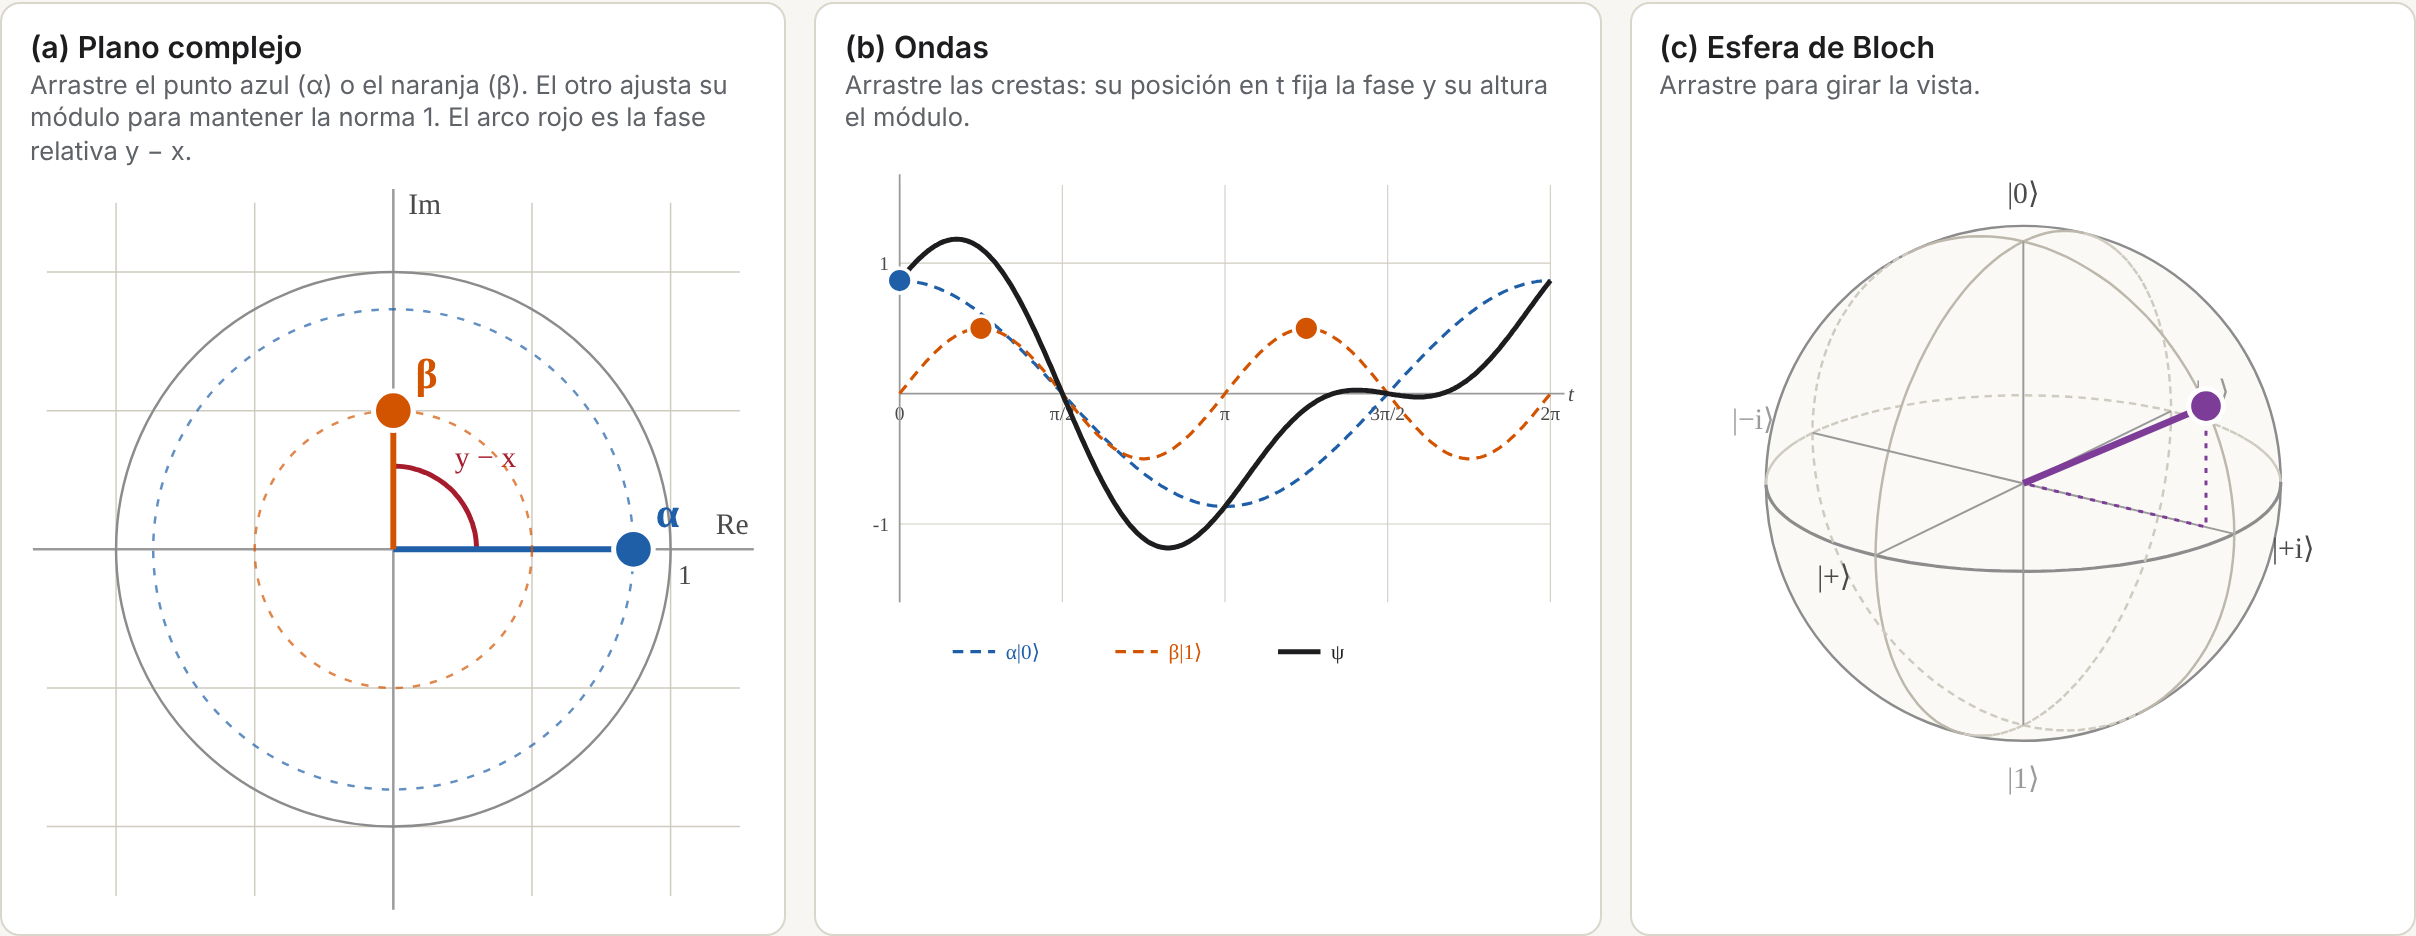
\includegraphics[width=\linewidth]{Imágenes/p13_widget_psi.png}
\caption{El estado $\ket\psi=\frac{\sqrt3}{2}\ket0+\frac{i}{2}\ket1$ en el widget del punto 1.2:
(a) los coeficientes, (b) las ondas y (c) el punto de la esfera de Bloch, con $\theta=60^\circ$
y $\varphi=90^\circ$.}
\label{fig:13-widget-psi}
\end{figure}

\begin{figure}[H]
\centering
\begin{minipage}{0.19\linewidth}\centering
  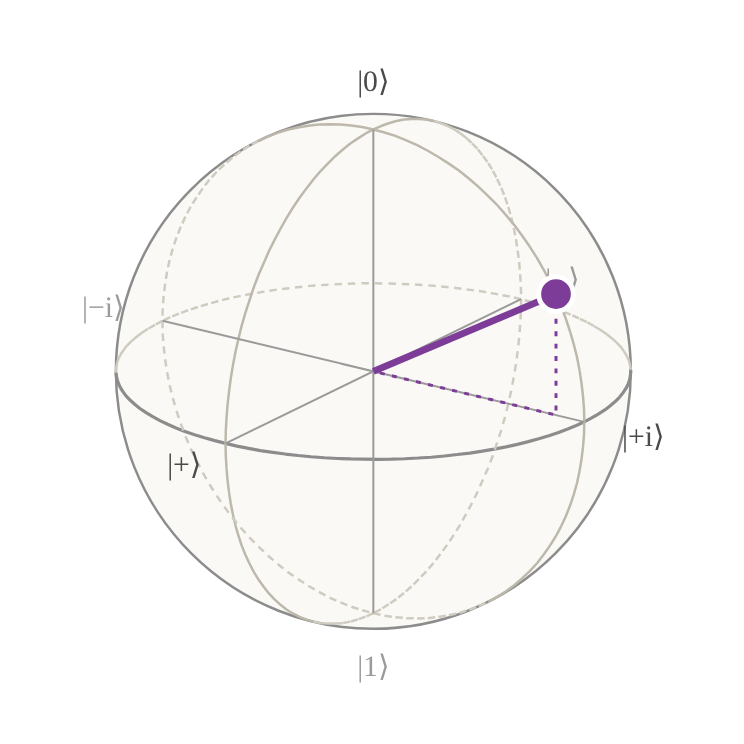
\includegraphics[width=\linewidth]{Imágenes/p13_bloch_psi.png}\\[-2pt]
  {\footnotesize $\ket\psi$\\ $\varphi=90^\circ$}
\end{minipage}\hfill
\begin{minipage}{0.19\linewidth}\centering
  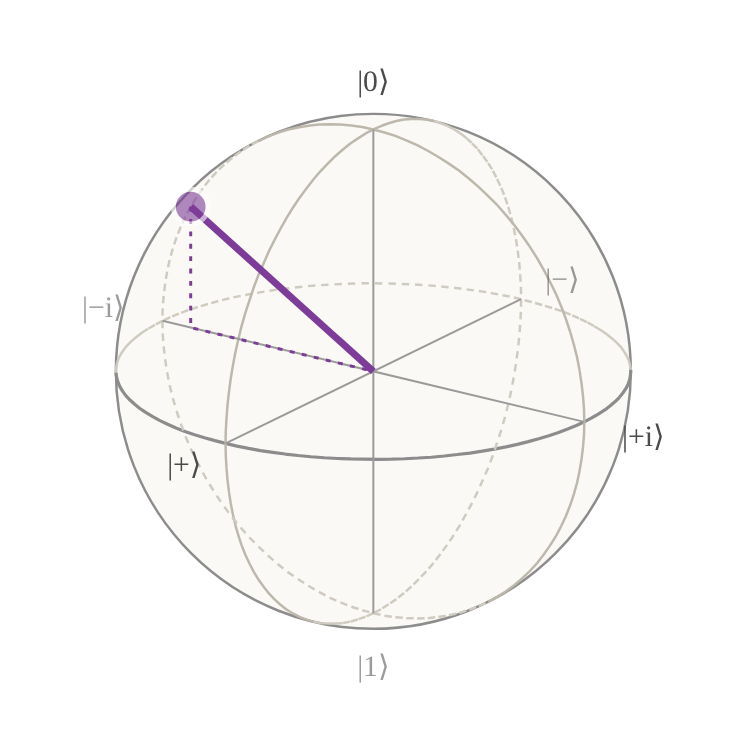
\includegraphics[width=\linewidth]{Imágenes/p13_bloch_tau0.png}\\[-2pt]
  {\footnotesize $\tau=0$\\ $\varphi'=-90^\circ$}
\end{minipage}\hfill
\begin{minipage}{0.19\linewidth}\centering
  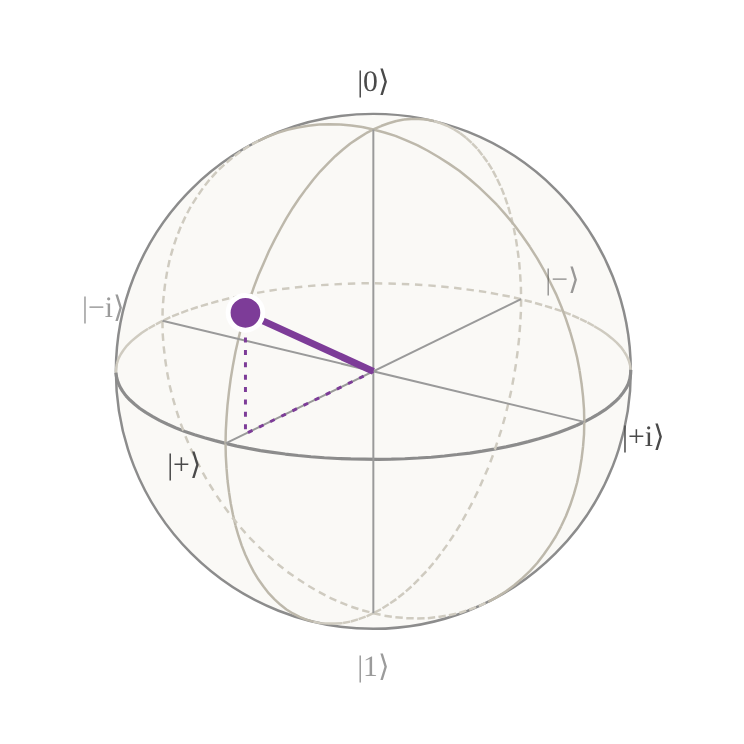
\includegraphics[width=\linewidth]{Imágenes/p13_bloch_taumas.png}\\[-2pt]
  {\footnotesize $\tau=\frac\pi2$\\ $\varphi'=0^\circ$}
\end{minipage}\hfill
\begin{minipage}{0.19\linewidth}\centering
  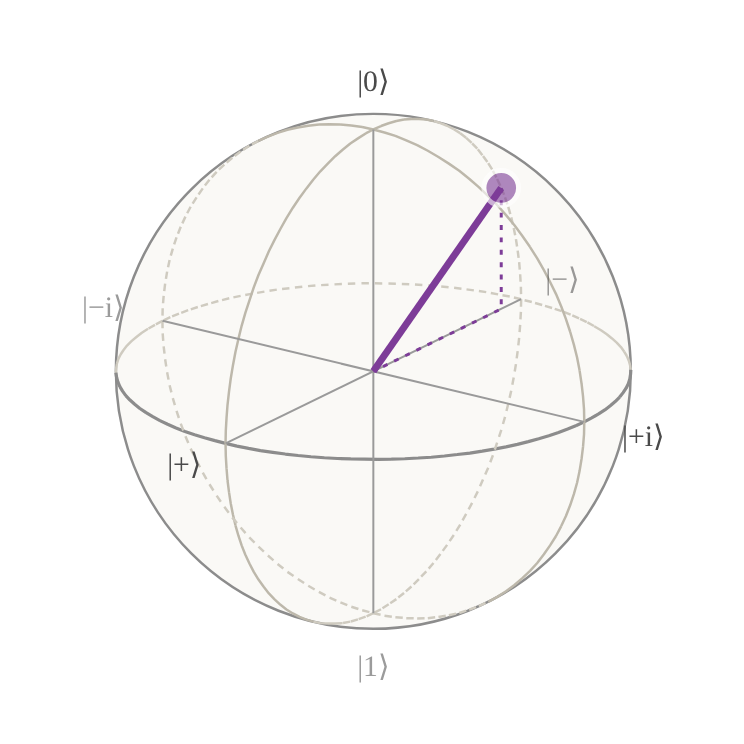
\includegraphics[width=\linewidth]{Imágenes/p13_bloch_taumenos.png}\\[-2pt]
  {\footnotesize $\tau=-\frac\pi2$\\ $\varphi'=180^\circ$}
\end{minipage}\hfill
\begin{minipage}{0.19\linewidth}\centering
  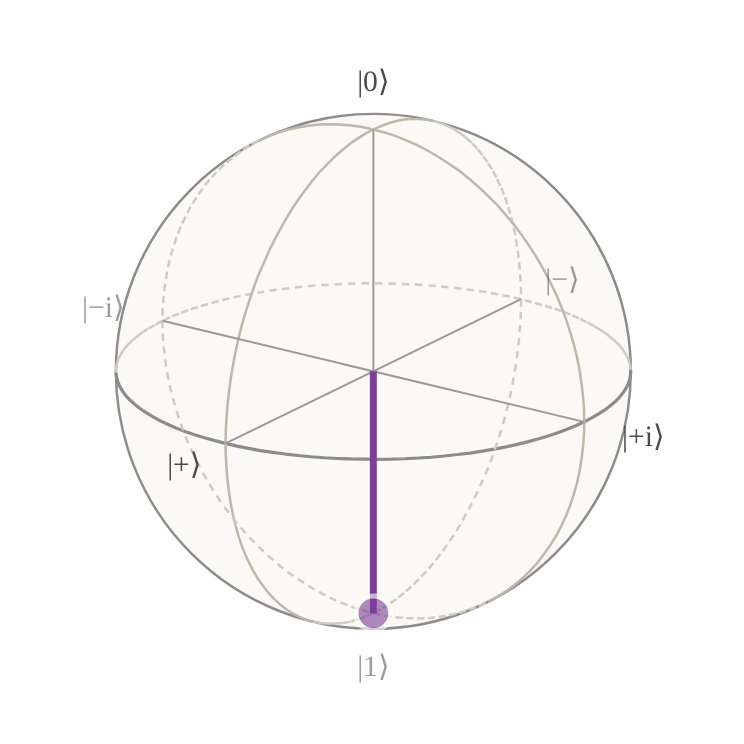
\includegraphics[width=\linewidth]{Imágenes/p13_bloch_final.png}\\[-2pt]
  {\footnotesize estado final\\ $\frac{c}{|c|}\ket1$}
\end{minipage}
\caption{$\ket\psi$, tres soluciones $\ket{\psi'}$ y el estado final en el widget. Los cuatro
primeros están en el mismo paralelo; el estado final es el polo sur.}
\label{fig:13-widget-bloch}
\end{figure}